\section{Adaptation}\label{badapt}
There are several styles of adaptation which affect both the possible application and the method of implementation. Firstly adaptation can be supervised in which case accurate transcriptions are available for all the adaptation data, or unsupervised in which case the required transcriptions must be hypothesis. Secondly, adaptation can be incremental, where adaptation data becomes available in stages or batch-mode, where all of the adaptation data is available from the start.\\
For cases where the adaptation data is limited, linear transform based schemes are currently the most effective form of adaptation. These approaches use the acoustic model parameters and require a transcription of the adaptation data.
\subsection{Maximum Likelihood linear Regression}\label{mllr}
In maximum likelihood linear regression (MLLR), a set of linear transformations are used to map and existing model set such that the likelihood of the adaptation data is maximized. \\
There are two main variants of MLLR:
\begin{itemize}
	\item Unconstrained MLLR: where separate transforms are trained for the means and variances. The effect of this transformations is to shift the component means and alter the variances in the initial system so that each state in the HMM system is more likely to generate the adaptation data.
	\item Constrained MLLR (CMLLR): where the transform for the mean and the variance is the same. The effect of this transformations is to shift the feature vector  in the initial system so that each state in the HMM system is more likely to generate the adaptation data.
\end{itemize}
CMLLR is the form of linear transform most often used for adaptive training even with little amount of adaptation data(\ref{articulo cmllr}). For both forms of linear transformation, the matrix transformation may be full, block-diagonal, or diagonal. CMLLR  is only implemented within HTK for diagonal covariance, continuous density HMMs due to computational reasons.

\subsection{Regression Class Trees}\label{rcs}
A powerful feature of linear transform-based adaptation is that it allows all the acoustic models to be adapted using a variable number of transforms. When the amount of data is limited, a global transform is applied to all the  Gaussian component in the model set, but as the amount of data increases, the HMM state components can be grouped into regression classes with each class having its own transform.\\
\begin{figure}[htb]
	\begin{center}
	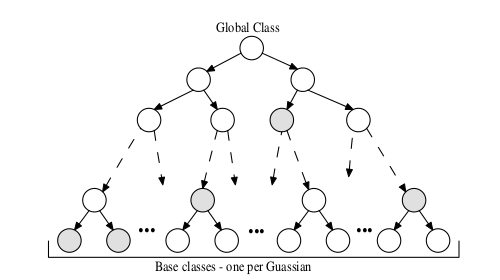
\includegraphics[width=1\textwidth]{img/RC2.png}
	\end{center}
	\caption{\label{rcimg}Regression class tree example \cite{hmmasr}}
\end{figure}
The number of transforms to use for any specific set of adaptation data can be determined automatically using regression class trees as illustrated in figure \ref{rcimg}. Each node represents a regression class (a set of Gaussian components that will share a single transform), the terminal nodes are called base classes. Then, for the given set of adaptation data, the tree is descended and the most specific set of nodes is selected for which there is enough data.
\subsection{Maximum a Posteriori}\label{map}
It is possible to use standard statistical approaches to obtain robust parameter estimates rather than looking for a form of transformation to represent the differences between speakers. This is what maximum a posteriori (MAP) adaptation does. In MAP a prior over the model parameters is used to estimate the model parameters in addition to the adaptation data.\\
MAP adaptation effectively interpolates the original prior parameter values with those that would be obtained from the adaptation data alone. As the amount of adaptation data increases, the adaptation gets better and closer to the adaptation domain.
\subsection{Adaptive Training}\label{at}
In the case of speaker independent, the training data includes large number of speakers. Therefore, training an acoustic model with different speakers "waste" a large number of parameters encoding the variability between speakers rather than the variability between spoken words which is the true aim. So what it can be done is to use adaptation transforms during the training step. This is known as speaker adaptive training (SAT).
\begin{figure} [htb]
	\begin{center}
	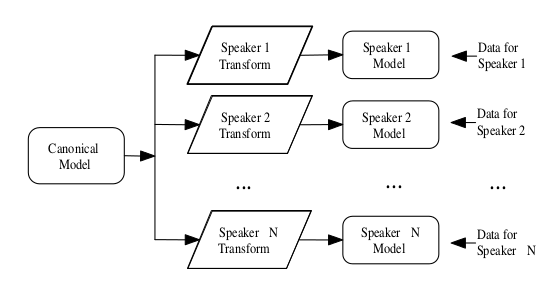
\includegraphics[width=1\textwidth]{img/sat2.png}
	\end{center}
	\caption{\label{satimg}Speaker adaptive training example \cite{hmmasr}}
\end{figure}
An example of this is illustrated in figure \ref{satimg}. For each training speaker a transform is estimated and then the canonical model is estimated given all of these speaker transforms. The complexity of this method depend of the nature of the adaptation transform that can be split in three groups \cite{hmmasr}
\begin{itemize}
	\item Model independent: These schemes do not make explicit use of any model information.
	\item Feature transformation: These transforms also act on the features but are derived, normally using ML estimation, using the current estimate of the model set.
	\item Model transformation: The model parameters, mean and possibly variances, are transformed.
\end{itemize}
The most common version of adaptive training uses CMLLR, since it is the simplest to implement.